\chapter{Construcción de bots mediante el DSL de SheetChat}

El diagrama de características estudiado previamente se ha de resolver en la definición de un chatbot. En este apartado se estudiará el DSL definido para la creación de un SheetChat. Para ello se tienen que tener en cuenta todas las características previamente mencionadas, la definición del origen de datos, la creación de una conversación que nos proporcione una petición de datos de entrada y su salida asociada; y no menos importante, recursos que nos permitan humanizar el bot para ofrecer una experiencia de usuario agradable.

Para ello en este trabajo se han elaborado tres ejemplos. El primero de ellos es dado las notas de dos asignaturas impartidas por un profesor de primaria, el poder preguntar por las notas de los alumnos que tiene. El segundo de los ejemplos permite dado un calendario de sesiones de un congreso científico, en este caso extraido del WISE de 2015\footnote{Calendario con las diferentes sesiones del congreso WISE: \url{http://www4.cis.fiu.edu/wise2015/@schema.html}}, poder obtener información sobre qué sesiones hay en los diferentes slots (u horarios). Por último, el tercer ejemplo permite, dada una hoja de cálculo autogenerada de una búsqueda de restaurantes de Miami en el sitio web Tripadvisor, obtener restaurantes por tipo de comida.

Cabe destacar que este DSL tiene múltiples objetivos:
\begin{itemize}
	\item El DSL debe ser fácilmente comprensible. Debe utilizar un lenguaje sencillo para la sintaxis concreta. En este caso se ha decidido implementarlo en JSON.
	\item El DSL debe de ser generable mediante una herramienta. La idea es que en un futuro este DSL sirva como base para una herramienta gráfica más sencilla de utilizar que ir escribiéndola de manera manual. Esto es debido al público objetivo, que son gente que desarrollan y utilizan hojas de cálculo en un dispositivo móvil; que carecerán de conocimiento de desarrollo de aplicaciones.
	\item El DSL debe permitir construir consultas complejas sin necesidad de hacer complejo el propio DSL.
	\item El DSL ha de abstraer de la implementación interna del bot y de las hojas de cálculo.
\end{itemize}

Partiendo de estas premisas, en la Figura \ref{fig:metamodel} se puede observar cuál es la sintaxis abstracta del DSL. Se define un SheetChat como una composición de un conjunto de Sheets y un Chat.

\begin{figure}[htb]
	\centering
	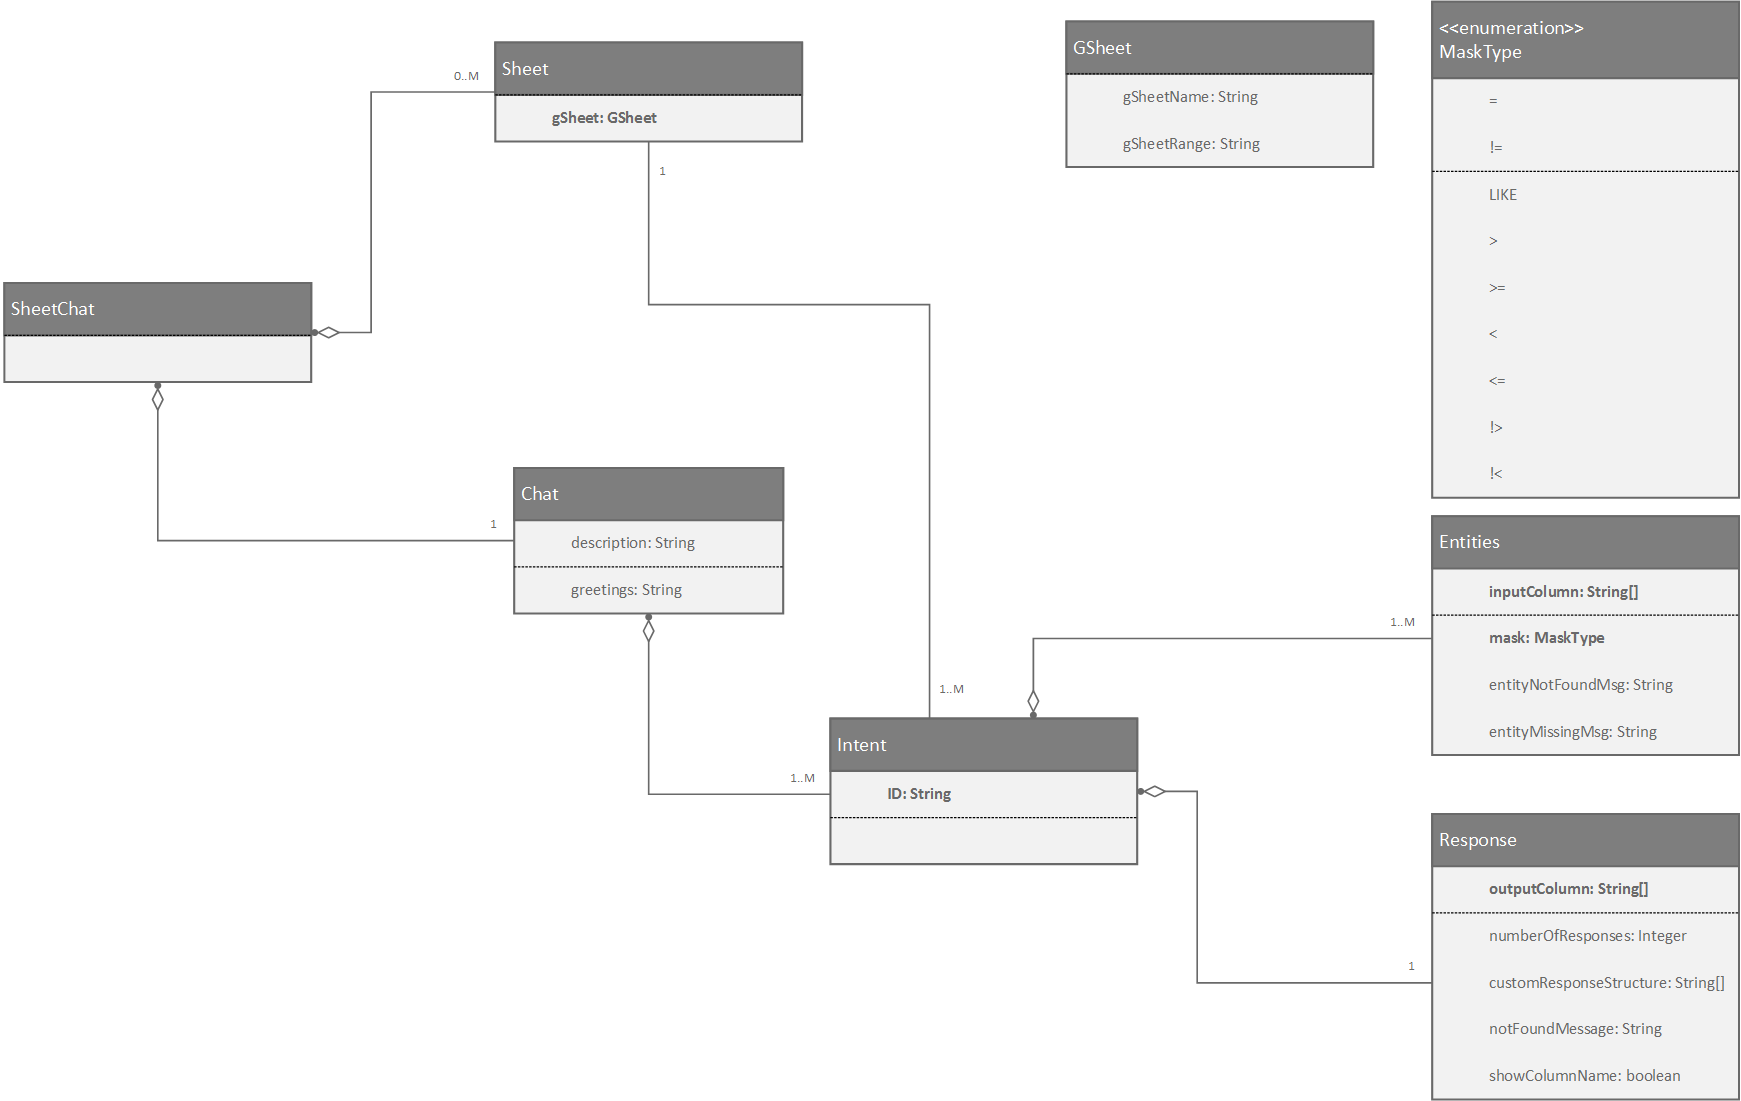
\includegraphics[width=0.8\textwidth]{./figs/Metamodel.png}
	\caption{Sintaxis abstracta del DSL para definir un SheetChat.} \label{fig:metamodel}
\end{figure}


Cada Sheet está representada por el nombre de la hoja de cálculo en Google SpreadSheets y el rango de las celdas que conforman la "tabla" sobre la que se consultará.

Cada Chat contendrá múltiples Intents. Cada uno de esos Intents tendrán un identificador único que estará relacionado con tipo de consulta que se le hará al Chatbot. Cabe destacar que los mensajes de Intents se infieren tras un entrenamiento a la herramienta Wit.ai mencionada en el Apartado \ref{sec:Humanization}. Por cada Intent habrá una respuesta que el chatbot proporcionará con el resultado extraído de la hoja de cálculo y un número de entidades que funcionarán a modo de filtrado para obtener ese resultado.

\section{Ejemplo 1: Notas de asignaturas impartidas por un profesor}

El uso de hojas de cálculo para almacenar las notas de los alumnos por parte del profesorado es una práctica habitual. Quizá un profesor no tenga una necesidad imperiosa de utilizar esta hoja de cálculo de manera móvil, pero es un ejemplo sencillo y claro para mostrar las características del DSL desarrollado.

La idea es que un profesor tenga 


\section{Ejemplo 2: Calendario de sesiones en un congreso científico}

Los congresos científicos aúnan conocimiento de distinta índole. Habitualmente estos eventos disponen de un calendario complejo, dónde hay trabajos más o menos interesantes o relevantes con la rama de especialización que tiene el asistente. Es por ello que acudir a las sesiones más afines a tu trabajo es importante. Es interesante disponer de información in situ de cuales son las próximas charlas que habrá, dónde o quién las presenta. Sin embargo, los sitios webs rara vez están preparados para su navegación por el móvil o se pierde mucho tiempo en encontrar los eventos a los que se desea acudir. Es una información relevante y que se desea conocer en el momento. 

En este ejemplo se trata de definir un Chatbot que permita consultar información relacionada con las diferentes sesiones de un congreso. Para ello el ejemplo se basa en extraer una tabla con el calendario del mismo y definir diferentes consultas sobre los datos. Para este ejemplo se han definido dos cuestiones habituales que suele tener un asistente a un congreso: 
\begin{itemize}
	\item \textbf{¿Cuáles son las charlas en un horario concreto, es decir, qué eventos hay en esa franja horaria?} De los eventos que existan en esa franja horaria, el asistente al congreso podría decantarse por la que más interesante le resulte.
	\item \textbf{¿Qué eventos hay relacionados con un tema (o topic) en particular?} De esta manera el usuario sabrá con una simple pregunta qué eventos le pueden resultar interesantes.
\end{itemize}



\section{Ejemplo 3: Búsqueda de restaurantes de Tripadvisor}

